% !TEX root = ./Basilisk-spacecraftPointing-20190116.tex


\section{Module Functions}

\begin{itemize}
    \item \textbf{Compute vector pointing to chief:} The inputs of the module are the location of the chief- and deputy spacecraft in the inertial frame. From these inputs, it is possible to calculate the vector that points from the deputy to the chief.
    \item \textbf{Compute the orientation of the reference frame with respect to the inertial frame:} After a coordinate system is built around the vector that points to the chief it is possible to determine the orientation of the reference frame with respect to the inertial frame.
    \item \textbf{Compute the angular velocity:} From the change in sigma over the timestep it is possible to compute the angular velocity of the reference frame.
    \item \textbf{Compute the angular acceleration:} Dividing the change in angular velocity of the reference frame over the timestep results in the angular acceleration.
\end{itemize}

\section{Module Assumptions and Limitations}

\begin{itemize}
    \item The user has to manually give a non-zero vector within the body frame as input. If this is not done an error occurs.
    \item Due to the fact that a numerical approximation is used for the determination of the angular velocity and the angular acceleration, the first two data points of the angular velocity and the first three data points for the angular acceleration are nonsense. For this reason, these are set to zero in the code.
    \item Due to the numerical method used the accuracy is heavily dependent on the timestep. This can be observed in Fig.~\ref{fig:att_error1}, Fig.~\ref{fig:att_error2}, and Fig.~\ref{fig:att_error3}. As the timestep decreases, the error decreases as well and smoothens out.
\end{itemize}

\begin{figure}[htb]
	\centerline{
	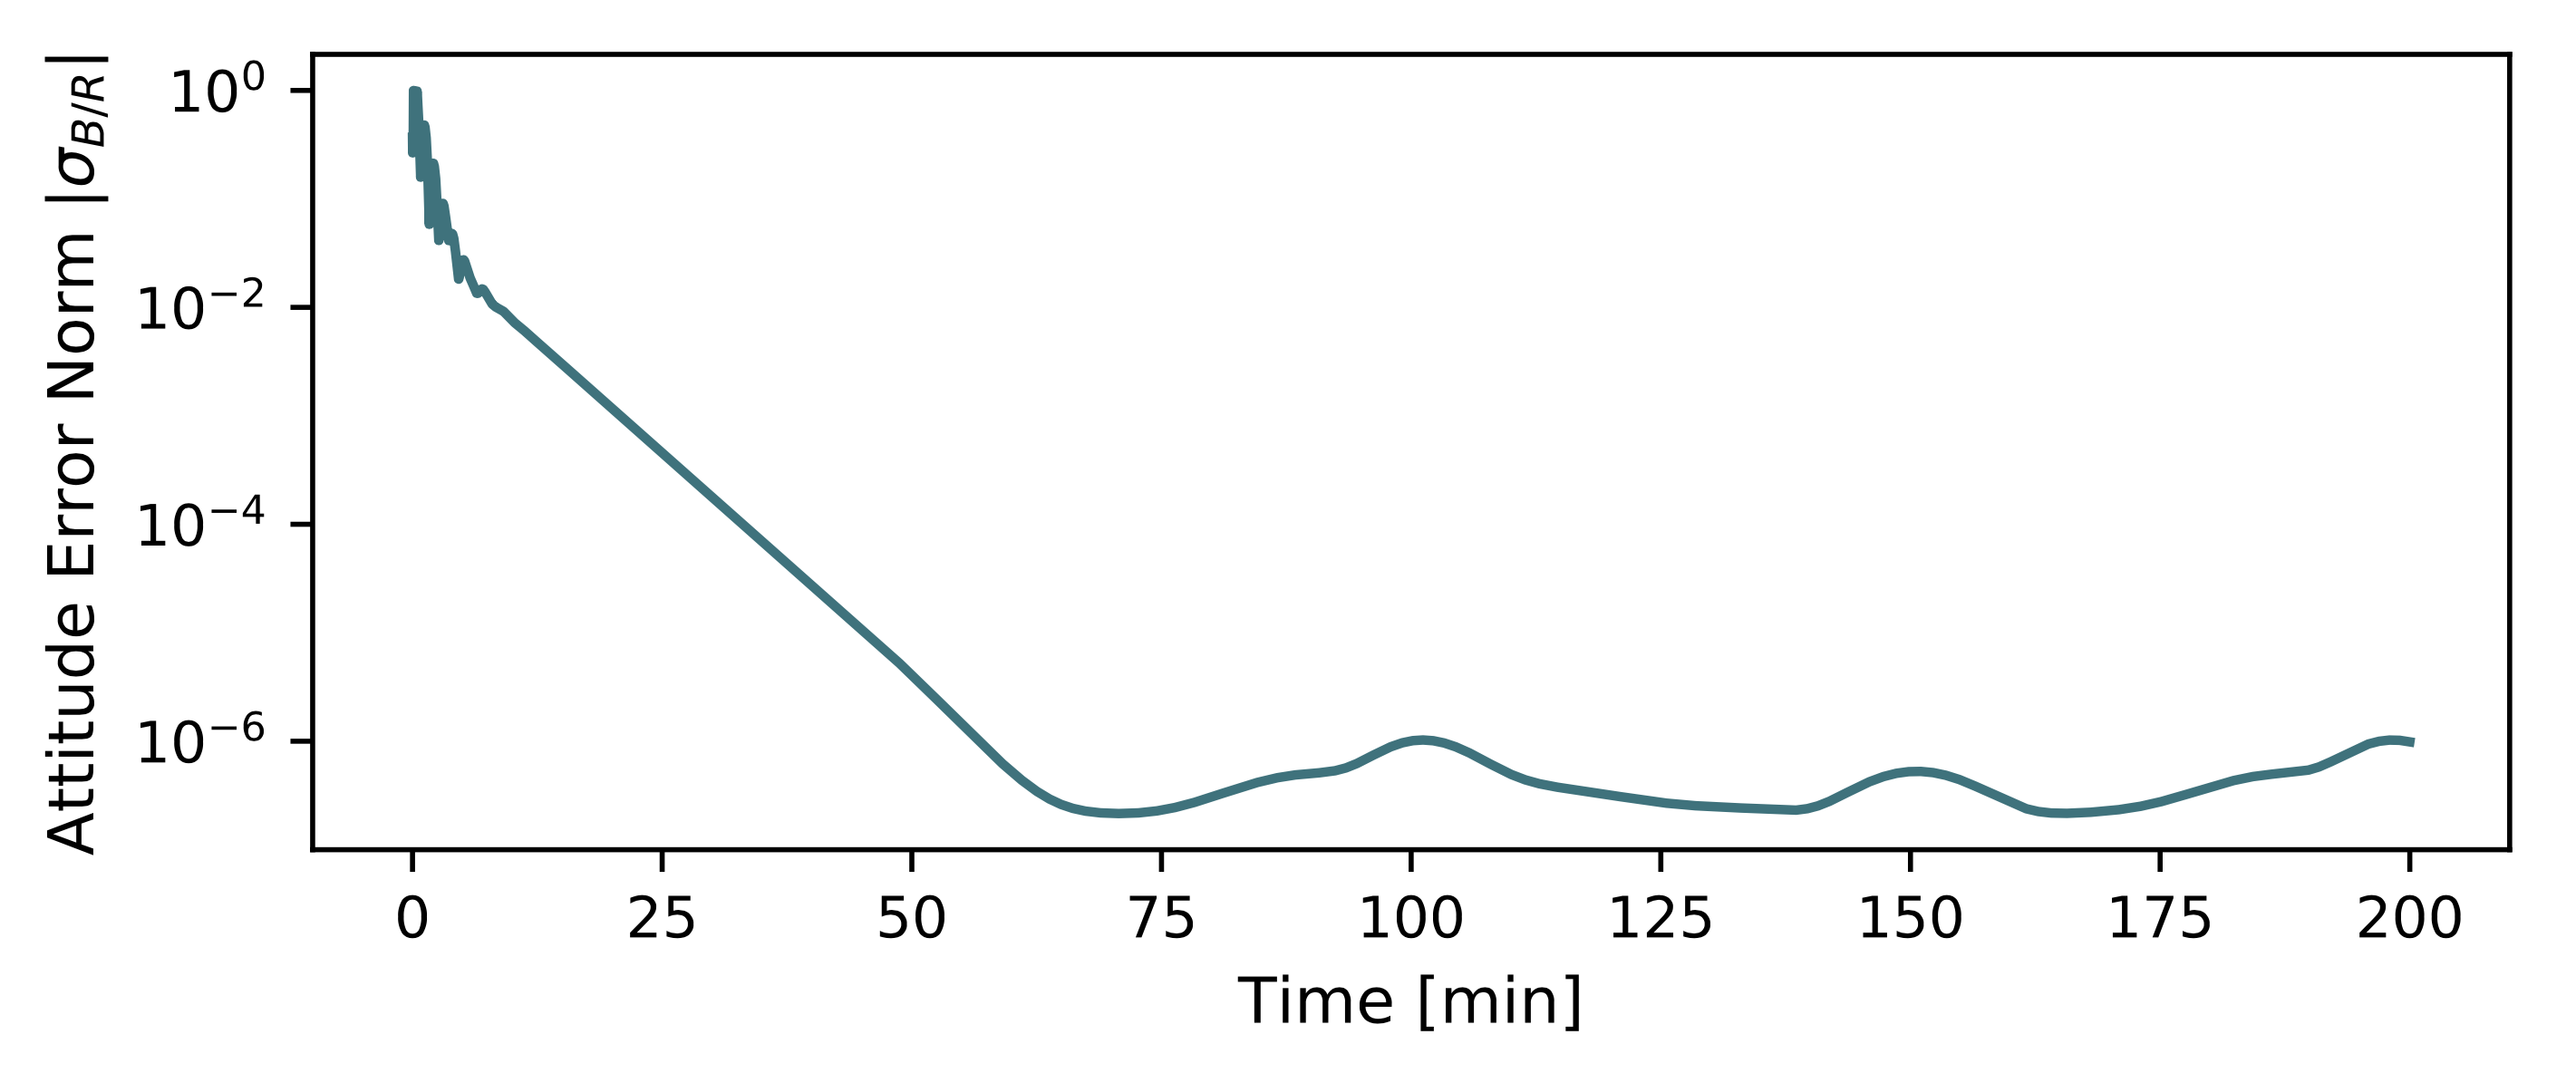
\includegraphics[scale=0.3]{Figures/att_norm1.png}
	}
	\caption{Timestep equal to 1s}
	\label{fig:att_error1}
\end{figure}

\begin{figure}[htb]
	\centerline{
	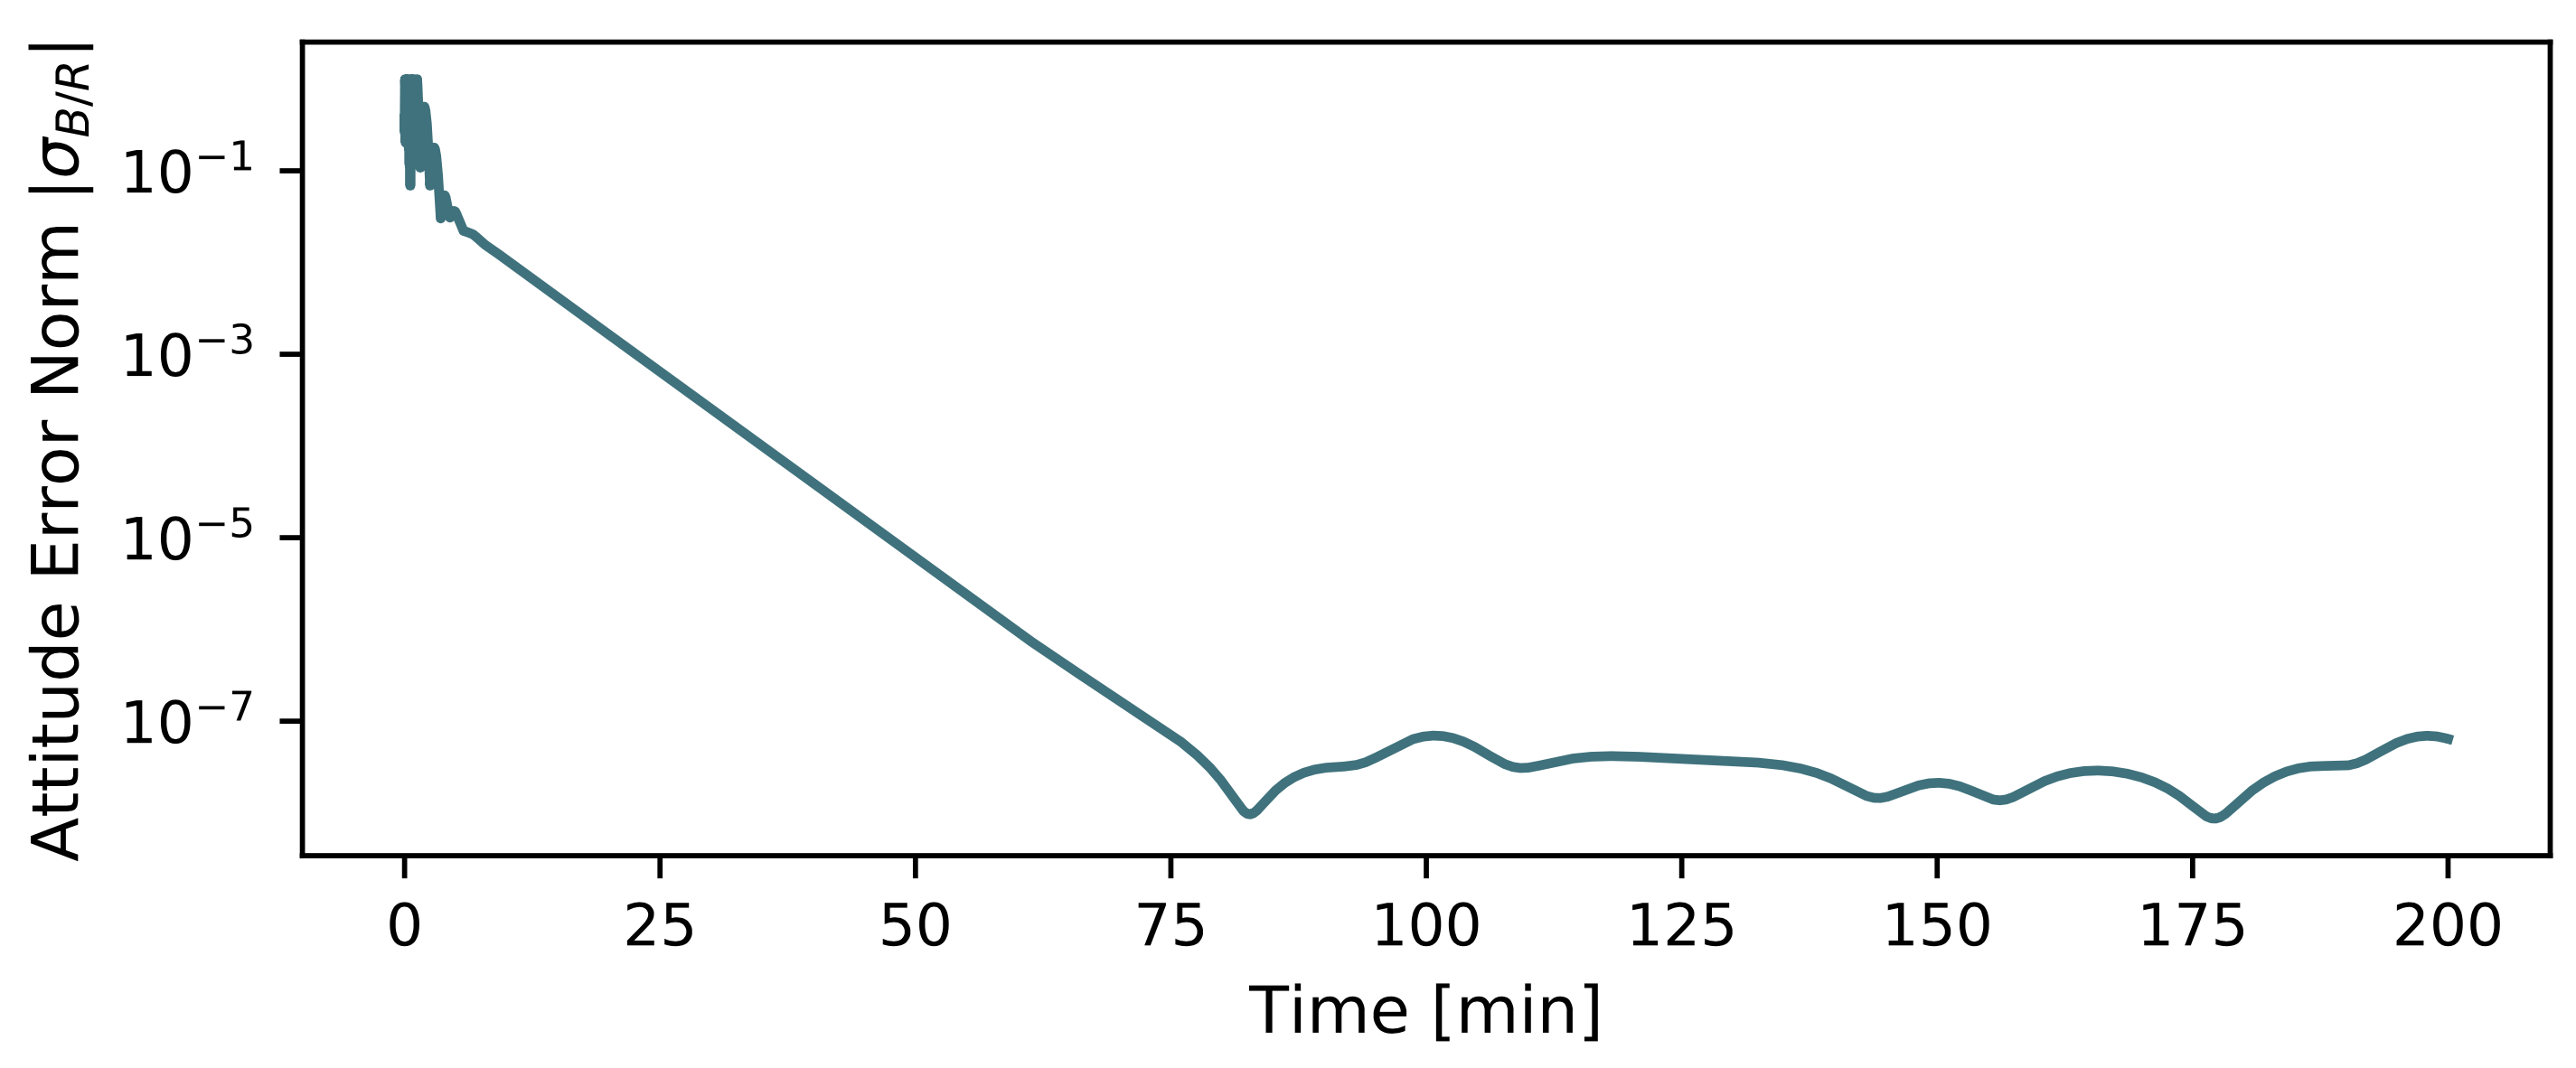
\includegraphics[scale=0.3]{Figures/att_norm2.png}
	}
	\caption{Timestep equal to 0.1s}
	\label{fig:att_error2}
\end{figure}

\begin{figure}[!htb]
	\centerline{
	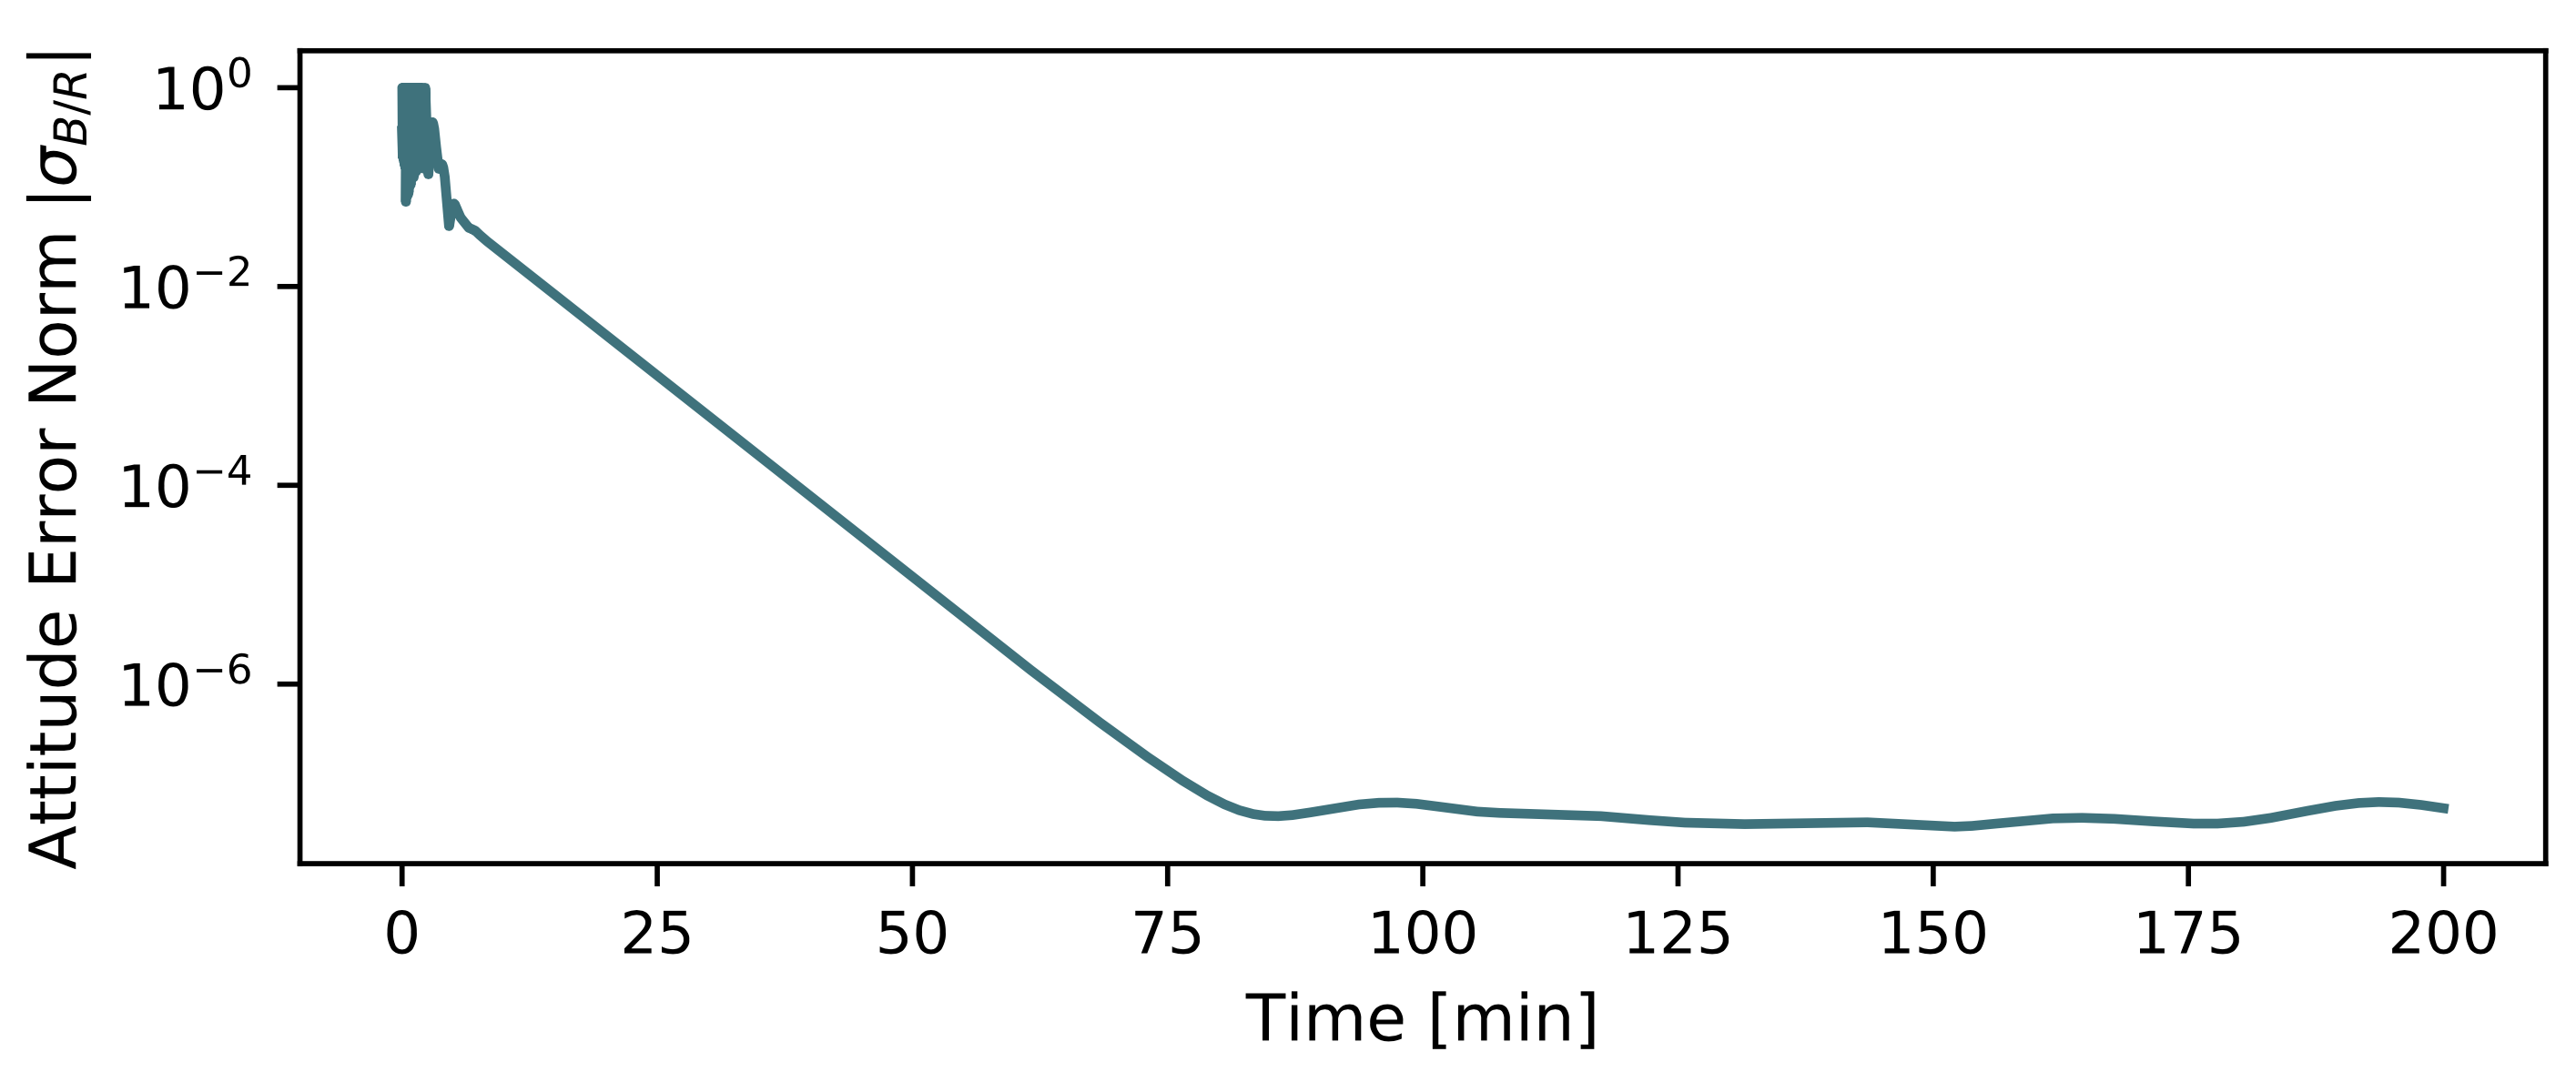
\includegraphics[scale=0.3]{Figures/att_norm3.png}
	}
	\caption{Timestep equal to 0.01s}
	\label{fig:att_error3}
\end{figure}


